\documentclass[10pt, letterpaper, headings=Large, DIV=14]{scrartcl}
% \usepackage{geometry}                % See geometry.pdf to learn the layout options. There are lots.
%\geometry{letterpaper}                   % ... or a4paper or a5paper or ... 
%\geometry{landscape}                % Activate for for rotated page geometry
%\usepackage[parfill]{parskip}    % Activate to begin paragraphs with an empty line rather than an indent
\usepackage{graphicx}
\usepackage{amssymb}
\usepackage{epstopdf}
\DeclareGraphicsRule{.tif}{png}{.png}{`convert #1 `dirname #1`/`basename #1 .tif`.png}

% \usepackage{titlesec}
% \titleformat{\subsection}[runin]{\sffamily \bfseries \large}{}{}{}[]
\renewcommand*{\titlepagestyle}{scrheadings}
\usepackage{palatino}
\usepackage{multicol}
\usepackage[]{natbib}
\bibstyle{apj}
\usepackage{amssymb}

\usepackage[usenames,dvipsnames,svgnames,html]{xcolor}
\usepackage{setspace}  % Needed for Double Spacing
\usepackage[english]{babel}
\usepackage{lipsum}

\DeclareGraphicsRule{.tif}{png}{.png}{`convert #1 `dirname #1`/`basename #1 .tif`.png}

\title{Galaxy evolution through the lens}  % add title here
%\author{T. Emil Rivera-Thorsen}  % include Author's name here
\date{}                                           % Activate to display a given date or no date

%%% BEGIN KOMASCRIPT
\setkomafont{title}{\large \sffamily \bfseries \color[HTML]{800000}}
\setkomafont{captionlabel}{\small \bfseries \sffamily}
\setkomafont{caption}{\footnotesize}
\setcapindent{1em}
\setkomafont{section}{\large \color[HTML]{800000}}
\setkomafont{subsection}{\normalsize \color[HTML]{000000}}
\setkomafont{author}{\small \itshape}
\setkomafont{pagenumber}{\large \upshape \bfseries \color[HTML]{FFFFFF}}
\usepackage[automark]{scrpage2}
\pagestyle{scrheadings}
\setheadsepline{.0pt}
\clearscrheadings
\automark[section]{chapter}
\ihead{\upshape \color[HTML]{999999} T. Emil Rivera-Thorsen}
\ohead{\colorbox[HTML]{800000}{\color{white} \pagemark}}
\chead{\upshape \color[HTML]{999999} Galaxy evolution through the lens}
\cfoot{}

%%% END KOMASCRIPT
\begin{document}

% \maketitle
\noindent {\color[HTML]{800000}\sffamily \bfseries \Large 
Star formation, feedback and Lyman $\alpha$ over cosmological time}
% \doublespacing

%\noindent
%\textbf{Title of Research Opportunity}: RO 18603: The Nature of Star-forming Galaxies at High Redshift\\
%\smallskip
% \noindent
% \textbf{Host institution}: Goddard Space Flight Center\\
% \smallskip
% \noindent
% \textbf{Host scientist}: Dr. Jane Rigby\\
% \smallskip
% 

\section*{Project overview}

{\bfseries \sffamily Main goal:} To investigate the nature of star-forming
galaxies in the epoch when the most stars in the Universe were formed (redshift
1-3), and how they compare to star forming galaxies in the local Universe,
ultimately attempting to disentangle intrinsic properties of the galaxies from
environmental differences over cosmological time spans. \newline

\noindent {\bfseries \sffamily Short outline:} We propose a two-pronged project
consisting of a local-Universe and a high-redshift part. In the local-universe
part, we propose to combine Hubble Legacy observations of various samples of
local star-forming galaxies, including but not limited to programs 11727, 13017
(PI Heckman), 12928 (PI Henry), 12539 (PI Bergvall), and 11522, 12027 (PI
Green), totalling an estimated 50 objects spanning a number of samples and
papers \citep[e.g.][]{Wofford2013,Alexandroff2015,Heckman2015,Henry2015}. The
idea is to give then a homogeneous treatment in inspired by the applicant's
earlier work on the Lyman Alpha Reference Sample \citep[LARS, ][]{LARSI,LARSII}
presented in \cite{RiveraThorsen2015} (hereafter RT15), to expand the coverage
of galaxy ages, masses etc. presented herein and provide a more statistically
solid basis for comparison. On top of this, data is currently being acquired
with HST of the nearby starburst ESO 338-04 (SAFE, GO 14806 PI: Östlin); 2
pointings with STIS and 12 pointings with COS, covering both hot central star
clusters and the outer, diffuse Ly$\alpha$ halo tracing (parts of) the galaxy's
neutral gas. Part of my project would be the analysis of these data, carrying
out a careful mapping and characterization of its ISM on a (coarsely) spatially
resolved basis.  

At high redshifts, I propose an analysis of spectroscopic rest-frame optical and
UV spectra from Project Megasaur (PI: Rigby), observed with Magellan/MagE and
Keck/ESI of 17 lensed, star-forming galaxies at $1 < z < 3$. The high
signal-to-noise ratio of these spectra, and the fact that the objects are
spatially resolved due to lensing, makes them ideal for bridging the gap between
high- and low-redshift samples: They have high enough redshifts for cosmological
evolution to be significant, while simultaneously being of high enough quality
that detailed analyses of Ly$\alpha$, stellar and nebular metal absorption
lines, nebular emission etc., like the ones done on the local samples, is
possible. Thus, a detailed, multi-parameter characterization is possible of
these objects, allowing to thoroughly evaluate differences and similarities
between these and the local objects.  The lensed spectra contain a wealth of
rest-frame NUV lines, including nebular emission in e.g. Mg \textsc{ii} and Fe
\textsc{ii} \citep[see e.g.][]{Bordoloi2016,Rigby2015}, which are typically not
included in the low-redshift HST-COS samples due to the detector range of the
COS. These lines are going to play a very important role in deep, high-redshift
galaxy surveys with the upcoming James Webb Space Telescope (JWST). With a
homogeneous, larger COS sample of local galaxies, and solid characterizations of
stellar populations, ISM kinematics etc. in hand, this knowledge can in turn be
used to calibrate our understanding and interpretation of the rest-frame NUV
line emission.  This project can therefore serve as a bridge between low and high
redshifts, as well as between the legacy of HST and the future of JWST. 


\section*{Background}

It is difficult to overestimate the importance of understanding star formation
and feedback for extragalactic astronomy in general. The majority of stars in
the Universe are formed during episodes of strong star formation, and the hot OB
population in these galaxies give rise to intrinsically strong Lyman $\alpha$
emission which is invaluable tools to probe e.g. the Universe's star formation
history, clustering properties and structure formation, marks the end of the
epoch of reinization, etc. However, since Ly$\alpha$ is resonantly scattered,
the photons travel much longer optical paths on their way out of the galaxy,
dramatically transforming thew line shape, morphology of the emerging radiation,
and dramatically increases the probability of being absorbed by dust grains on
the way. These effects can be countered by a number of other mechanisms, e.g.
bulk outflows, low dust content, low kinematic line width, low neutral gas
covering fraction and column density, high clumpiness of the neutral medium, and
more (see RT15) for details). Also the reionization and reheating of the early
Universe is believed to be driven in large part by star-forming galaxies,
however, to do so, enough ionizing photons must not only be produced, but also
be able to escape into the intergalactic medium, which does not seem to be
possible if conditions in the galaxies at the time were like at present. It is
clear that a strong evolution must have happened, and Ly$\alpha$ studies can
help us understand this evolution. We have recently begun to understand how
Ly$\alpha$ and Lyman Continuum partially escapes through the same channels, and
how to read information about the neutral medium important for Lyman Continuum
escape from Ly$\alpha$ profiles\citep{Verhamme2015}.  More importantly; the
correct understanding of Ly$\alpha$ emission is also important to infer the true
luminosity function of galaxies in the Universe from the one we observe in
Ly$\alpha$.  

Lyman $\alpha$ is not the only important emission line in this
wavelength range. As we venture into the neutral epoch of the Universe
(redshifts $\gtrsim 7$), as will be possible with the launch of the James Webb
telescope, the IGM suppresses Ly$\alpha$ strongly \citep[e.g.][and
references herein]{Laursen2009,Dijkstra2006,DijkstraRev}.  However, with the
strongly improved sensitivity that will be at our disposal with JWST, other
nebular emission lines in the rest-frame NUV can gain importance as beacons.
However, it's been shown by \cite{Rigby2014} that the emission of Mg II 2796,
2803 does not correlate with that of Ly$\alpha$, implying that a more thorough
understanding of the origin of these NUV lines is necessary to correctly
understand and compare observations of these to more nearby surveys based on
Ly$\alpha$ luminosities. 

This proposed project aims to (A).\ consolidate our
current knowledge of the connections between kinematics and Ly$\alpha$ transfer
and escape in the local Universe; to (B) create grounds for direct comparison
between these and the galaxies at high redshift, and finally (C) by the aid of
(A) and (B), investigate the connection between kinematics and other ISM
features, Ly$\alpha$, and NUV metal emission, and thus pave the road for
future JWST-based surveys to be more easily understood in the context of current
knowledge. \newline




\noindent{\sffamily \bfseries Project Megasaura} (PI J. Rigby) is a sample of 17 strongly lensed, star
forming galaxies at redshifts between 1 and 3 which have been observed in the
optical, NIR and MIR with Magellan/MagE and Keck/ESI, and imaged by HST and
Spitzer.  The strong lensing gives an unusually fine signal-to-noise, allowing detailed
studies in both emission and absorption lines. In itself, the sample is a unique
opportunity to study star forming galaxies in the epoch where the majority of
stars in the Universe were formed; but furthermore, it allows testing of the
detailed knowledge of local-Universe star forming galaxies which has
been obtained within the last decade, on data from an entirely different epoch
but of comparable quality. Such a comparison could potentially disentangle
intrinsic, evolutionary changes over cosmological time, from changes in the
environment, and help understand star formation, galaxy evolution, and
Ly$\alpha$ transfer and escape both locally and in the early Universe.
I propose at least two sub-projects centered on this sample: \textbf{The first}
will consist of a general characterization of the objects wrt.\ age, mass,
stellar population, SFR etc., in order to establish a baseline towards future
results can be compared; and furthermore, it will contain an analysis of
kinematics in the ISM and a comparison to properties in Ly$\alpha$. 
Where possible, I have been granted permission to fit the Ly$\alpha$ emission
profiles against the grid of semi-analytical expanding-shell models developed by
the expert group at Geneva Observatory \citep{Scharer2011}, which I believe
could add significant value to these kinematic analyses in terms of
comparability to local-Universe galaxies. It is the hope that this will enable
us to test the insights obtained from local samples in a high-redshift setting,
and possibly reveal systematic differences between local and high-redshift galaxies.
\textbf{The second} proposed paper on
Project Megasaura will be focused on NUV nebular and stellar emission lines of
e.g. Fe \textsc{ii}, Mg\textsc{ii}, and C \textsc{iii}], and the connection
between their line profiles, line strength etc. to stellar and kinematic ISM
properties. The hope is, besides learning more about the individual galaxies,
could help calibrate these NUV emission lines as a tool for future cosmology. 
If there should be time over, looking deeper into the spatially
resolved subsets of the sample and spatially mapping choice properties should be
interesting, and holds the possibility of comparisons to the low-redshift SAFE
project (see below). 
Fig.~\ref{fig:mega} shows an example finding chart of MagE observations of one
of the Megasaura (left), and a curve of running averaged signal/noise per pixel
of this and two other spectra.  \newline



\noindent {\bfseries \sffamily The Lyman Alpha Reference Sample}: is a
sample of originally 14 galaxies (since extended with 28 galaxies
more, the analysis of which is still underway), established with the goal of
studying local-Universe analogs of high-redshift star-forming galaxies in as
great detail as possible in order to learn which mechanisms govern Ly$\alpha$
radiative transfer and escape. The sample has been observed with a large range of
instruments and wavelength ranges, from archival X-Ray data from Chandra and
XMM, to 21 cm eVLA interferometry. The back bone is a set of multi-band HST ACS 
and WFC3 imaging and COS spectroscopy. My main contribution to this project has
been the analysis of these COS spectra, published in RT15. Through this work, I
have gained a deep and highly specialized knowledge of the atomic and ionized
ISM in these galaxies, its kinematics and geometry, and its interplay with the
Ly$\alpha$ photons. 
Fig.~\ref{fig:LARS} shows some core results from LARS in spectroscopy. In the
left panel is the results of AOD computations for one of the galaxies, more
closely explained in the caption. In the middle panel is shown a plot of
EW(H$\alpha$) vs.\ maximum velocity-binned neutral covering fraction in the sample
galaxies (see RT15 for more detail). Here, we found strong correlation,
suggesting that strong SF feedback perforates the surrounding neutral medium,
carving pathways for Ly$\alpha$ to escape. Testing whether this correlation
holds for a larger sample is one of the motivations for the HST Legacy
sub-project. Right panel shows observed Ly$\alpha$ of LARS 1, together the
best-fit model of the Geneva grid, and intrinsic Ly$\alpha$ as traced by
H$\alpha$.  We also propose a similar Ly$\alpha$ profile analysis in this larger
COS Legacy sample and for the Megasaura for which Ly$\alpha$ emission strength
and S/N allows it. 

\textbf{The third proposed paper} will consist of running a larger number of
archival COS observations of local star forming galaxies (see the first page for
suggested proposal IDS) through the same
machinery as was the LARS, to provide a stronger statistical reliability and a
larger population coverage to the sample, such that a wider variety of
star-forming galaxies at high redshifts have as close and statistically sound
representation in the sample as possible. This would help consolidate our
current knowledge about local Universe conditions, and to draw conclusions about
similarities to and differences from the high redshift Universe with much
stronger confidence.  \newline 



\noindent
{\bfseries \sffamily SAFE --- Star clusters, lyman-Alpha, and Feedback in Eso
338-04: } Star forming or starburst galaxies are often messy, strongly interacting
systems with complex kinematics and a strong internal variation in stellar
population, star formation activity etc., as has often been shown in the
literature at  low redshifts; and e.g. \cite{Bayliss2014} show that this can
also be the case with lensed, high-$z$ galaxies. This presents challenges to
both observing and modelling them. 
SAFE is an attempt to map both star clusters, neutral and ionized ISM, intrinsic
and emerging Ly$\alpha$ and other properties across an entire galaxy in the UV -
something that would normally be done with an IFU in the optical. For lack of
space-borne IFUs, however, this is an attempt to essentially turn the COS into a
coarse-grained one. It was originally devised as a means to create a realistic
input for Ly$\alpha$ radiative transfer simulations, but the insights it will
bring should be interesting to the broader star-forming galaxy community in many
ways, as is hinted by \cite{Bayliss2014}. 
\textbf{ A fourth subproject} will be to work on SAFE. The project includes a
large amount of data, and there will be a lot to do, but the work can be broken
into smaller portions. Should the assignment grow from 2 to 3 years, SAFE holds
enough data and complexity to take up a significant part of a third year, but
some of the more low-hanging fruit like Ly$\alpha$ profile mapping over spatial
regions can most likely be packed into a smaller project of a shorter time span. 

\section*{Timeline}

\begin{description}
	\item[Months 1-5] \emph{Local HST Legacy COS galaxies}. Much of the
		computational machinery for this is already in place; so the
		core analysis of this should be relatively straightforward. 
	\item[Months 6-14] \emph{Megasaura I}. This paper will contain a relatively
		large number of measurements and diagnostics, and likely a
		nontrivial amount of data reduction/combination etc., and will
		require a considerable amount of work.
	\item[Months 15-20] \emph{Megasaura II}. The proportions of the two Megasaura
		papers is uncertain, but a total of 14 months for both seems
		realistic. 
	\item[Months 16-24] \emph{SAFE}. This project contains material for large
		amounts of work, but can be split up into smaller parts. If the
		position gets extended to a third year, SAFE can very well
		expand to fill a large chunk of this .
	\item[Months 25-?] If the assignment expands to a third year, the option
		should be kept open that results from the first two years could
		lead to exciting questions. Otherwise, SAFE is likely to hold
		data enough for a good part of this, and a comparison to the
		spatially resolved Megasaurs could be interesting. 
\end{description}

\bibliographystyle{aasjournal}
\begin{scriptsize}
	\bibliography{thesis}
\end{scriptsize}

\section*{Figures}

\begin{figure}[h] %  figure placement: here, top, bottom, or page
   \centering
   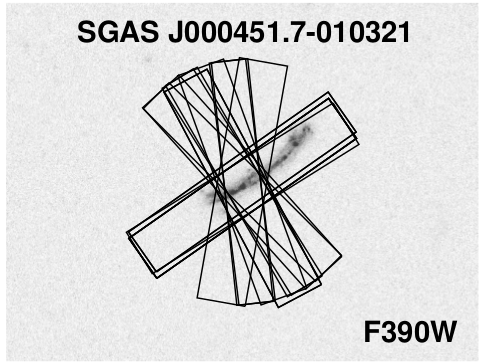
\includegraphics[width=0.39\textwidth]{MegasaurExample.png}
   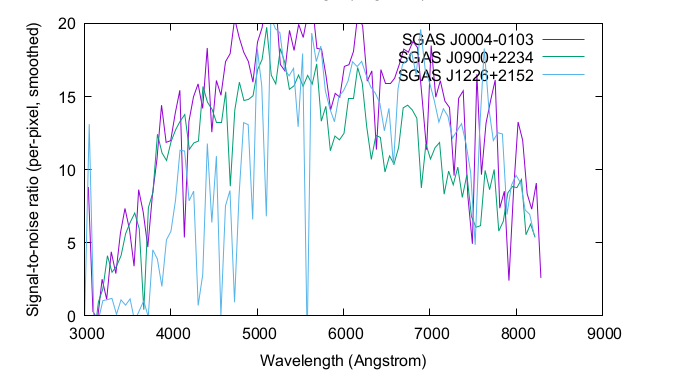
\includegraphics[width=0.59\textwidth]{SNRs.png} 
   \caption{\small Example finding chart for Magellan/MagE observations of a Megasaur
	   (left), and averaged SNR per pixel in the combined spectra of same
	   galaxy (purple) and two other sample galaxies (right). Images 
	   provided by J. Rigby.}
   \label{fig:mega}
\end{figure}


\begin{figure}[h] %  figure placement: here, top, bottom, or page
   \centering
   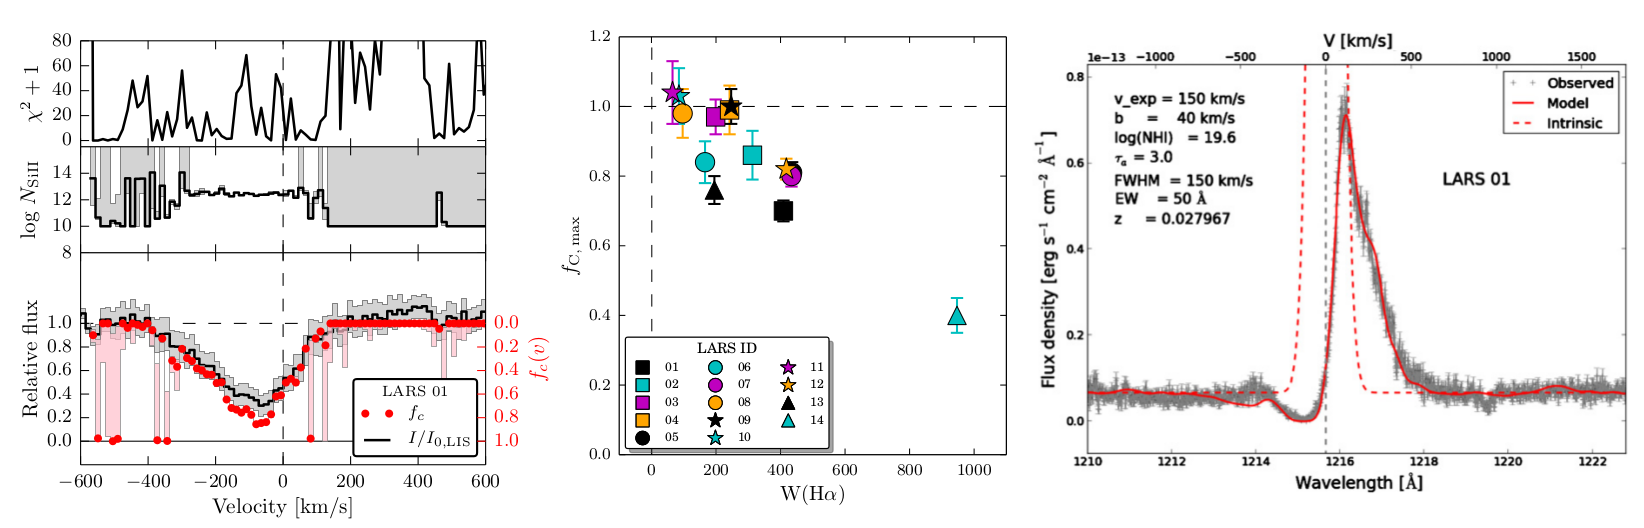
\includegraphics[width=\textwidth]{LarsResults.png} 
   \caption{\small eft: Result of Apparent Optical Depth analysis of a LARS galaxy.
   Middle panel shows inferred column densities with errors, lower panel
   shows computed per-bin covering fractions, overlaid on the
   averaged LIS metal absorption profile; from RT15. Center: H$\alpha$ EW vs.
   Maximum covering fraction for the LARS galaxies; from RT15. Right: Ly$\alpha$
   profile of LARS 1 (black), with intrinsic Ly$\alpha$ inferred from H$\alpha$
   (dotted red) and the best-fit model from the catalog of the Geneva group
   (Orlitova et al, in prep.), from \cite{LARSI}.}
   \label{fig:LARS}
\end{figure}


\begin{figure}[h] %  figure placement: here, top, bottom, or page
   \centering
   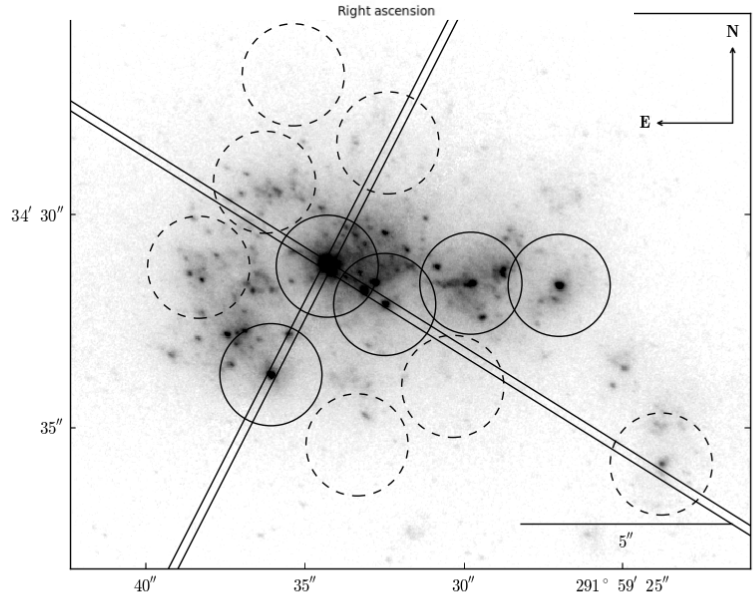
\includegraphics[width=0.7\textwidth]{SAFEpointings.png} 
   \caption{STIS and COS pointings for the SAFE project., overlaid on HST UV
   continuum image of ESO 338-04. Image from SAFE proposal by Östlin.}
   \label{fig:example}
\end{figure}

% \begin{figure}[h] %  figure placement: here, top, bottom, or page
%    \centering
%    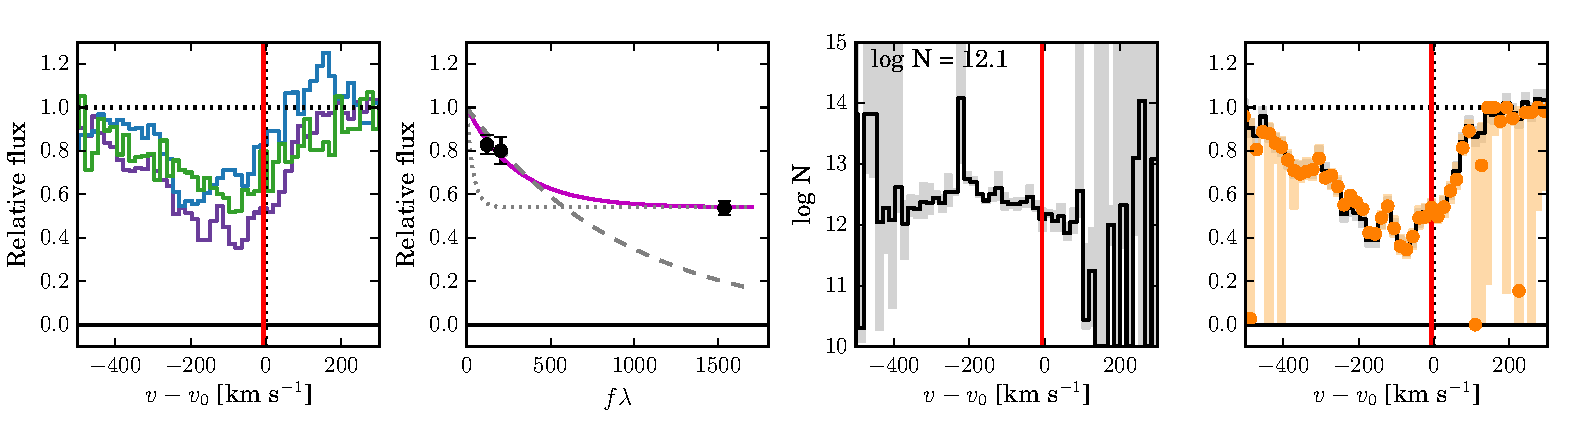
\includegraphics[width=\textwidth]{../../../Haro11Cos/Figs/AOD-details-example-4pane.pdf} 
%    \caption{Illustration of the AOD method with example data from Haro 11.
%    \textbf{Far left}: Line profile of Si\textsc{ii}\(\lambda\lambda 1260, 1304,
%    1526\), and a vertical red line denoting the velocity bin of interest for the
%    example. \textbf{Center left}: Residual intensity as a function of
%    \(f\lambda\) for the three lines. The best fit of \(I/I_0(f\lambda)\) is 
%    shown in magenta. In gray is shown for illustration \(I/I_0\) in the extreme
%    cases of \emph{a)} unchanged $f_C$ but much higher $N$ (dotted) or \emph{b)}
%    $f_C=1$ and $N$ 0.5 dex lower. \textbf{Center right}: $\log N$ as function of
%    $v$ for these profiles, and \textbf{far right}: $1-f_C$ as function of v
%    (orange circles) superimposed on the profile of Si \textsc{ii} 1260 (black
% 	   steps). Shaded regions are standard errors. }
%    \label{fig:example}
% \end{figure}


\end{document}  
